% Options for packages loaded elsewhere
\PassOptionsToPackage{unicode}{hyperref}
\PassOptionsToPackage{hyphens}{url}
\PassOptionsToPackage{dvipsnames,svgnames,x11names}{xcolor}
%
\documentclass[
  10pt,
  ignorenonframetext,
]{beamer}
\usepackage{pgfpages}
\setbeamertemplate{caption}[numbered]
\setbeamertemplate{caption label separator}{: }
\setbeamercolor{caption name}{fg=normal text.fg}
\beamertemplatenavigationsymbolsempty
% Prevent slide breaks in the middle of a paragraph
\widowpenalties 1 10000
\raggedbottom
\setbeamertemplate{part page}{
  \centering
  \begin{beamercolorbox}[sep=16pt,center]{part title}
    \usebeamerfont{part title}\insertpart\par
  \end{beamercolorbox}
}
\setbeamertemplate{section page}{
  \centering
  \begin{beamercolorbox}[sep=12pt,center]{part title}
    \usebeamerfont{section title}\insertsection\par
  \end{beamercolorbox}
}
\setbeamertemplate{subsection page}{
  \centering
  \begin{beamercolorbox}[sep=8pt,center]{part title}
    \usebeamerfont{subsection title}\insertsubsection\par
  \end{beamercolorbox}
}
\AtBeginPart{
  \frame{\partpage}
}
\AtBeginSection{
  \ifbibliography
  \else
    \frame{\sectionpage}
  \fi
}
\AtBeginSubsection{
  \frame{\subsectionpage}
}
\usepackage{amsmath,amssymb}
\usepackage{iftex}
\ifPDFTeX
  \usepackage[T1]{fontenc}
  \usepackage[utf8]{inputenc}
  \usepackage{textcomp} % provide euro and other symbols
\else % if luatex or xetex
  \usepackage{unicode-math} % this also loads fontspec
  \defaultfontfeatures{Scale=MatchLowercase}
  \defaultfontfeatures[\rmfamily]{Ligatures=TeX,Scale=1}
\fi
\usepackage{lmodern}
\usetheme[]{metropolis}
\ifPDFTeX\else
  % xetex/luatex font selection
\fi
% Use upquote if available, for straight quotes in verbatim environments
\IfFileExists{upquote.sty}{\usepackage{upquote}}{}
\IfFileExists{microtype.sty}{% use microtype if available
  \usepackage[]{microtype}
  \UseMicrotypeSet[protrusion]{basicmath} % disable protrusion for tt fonts
}{}
\makeatletter
\@ifundefined{KOMAClassName}{% if non-KOMA class
  \IfFileExists{parskip.sty}{%
    \usepackage{parskip}
  }{% else
    \setlength{\parindent}{0pt}
    \setlength{\parskip}{6pt plus 2pt minus 1pt}}
}{% if KOMA class
  \KOMAoptions{parskip=half}}
\makeatother
\usepackage{xcolor}
\newif\ifbibliography
\usepackage{listings}
\newcommand{\passthrough}[1]{#1}
\lstset{defaultdialect=[5.3]Lua}
\lstset{defaultdialect=[x86masm]Assembler}
\usepackage{graphicx}
\makeatletter
\def\maxwidth{\ifdim\Gin@nat@width>\linewidth\linewidth\else\Gin@nat@width\fi}
\def\maxheight{\ifdim\Gin@nat@height>\textheight\textheight\else\Gin@nat@height\fi}
\makeatother
% Scale images if necessary, so that they will not overflow the page
% margins by default, and it is still possible to overwrite the defaults
% using explicit options in \includegraphics[width, height, ...]{}
\setkeys{Gin}{width=\maxwidth,height=\maxheight,keepaspectratio}
% Set default figure placement to htbp
\makeatletter
\def\fps@figure{htbp}
\makeatother
\setlength{\emergencystretch}{3em} % prevent overfull lines
\providecommand{\tightlist}{%
  \setlength{\itemsep}{0pt}\setlength{\parskip}{0pt}}
\setcounter{secnumdepth}{-\maxdimen} % remove section numbering
\ifLuaTeX
\usepackage[bidi=basic]{babel}
\else
\usepackage[bidi=default]{babel}
\fi
\babelprovide[main,import]{american}
% get rid of language-specific shorthands (see #6817):
\let\LanguageShortHands\languageshorthands
\def\languageshorthands#1{}
\usepackage{fancyhdr}
\pagestyle{fancy}
\usepackage{setspace}
\usepackage{graphicx}
\usepackage{amsfonts}
\usepackage{amssymb}
\usepackage{amsmath}
\usepackage{minted}
\ifLuaTeX
  \usepackage{selnolig}  % disable illegal ligatures
\fi
\IfFileExists{bookmark.sty}{\usepackage{bookmark}}{\usepackage{hyperref}}
\IfFileExists{xurl.sty}{\usepackage{xurl}}{} % add URL line breaks if available
\urlstyle{same}
\hypersetup{
  pdftitle={Understanding Memory Management},
  pdfauthor={Dipesh Kafle},
  pdflang={en-US},
  colorlinks=true,
  linkcolor={blue},
  filecolor={Maroon},
  citecolor={Blue},
  urlcolor={red},
  pdfcreator={LaTeX via pandoc}}

\title{Understanding Memory Management}
\author{Dipesh Kafle}
\date{}

\begin{document}
\frame{\titlepage}

\begin{frame}
\setsansfont[ItalicFont={Fira Sans Light Italic},%
BoldFont={Fira Sans SemiBold},%
BoldItalicFont={Fira Sans Italic}]%
{Fira Sans Light}\%
\end{frame}

\begin{frame}{Memory Layout}
\protect\hypertarget{memory-layout}{}
\begin{figure}
\centering
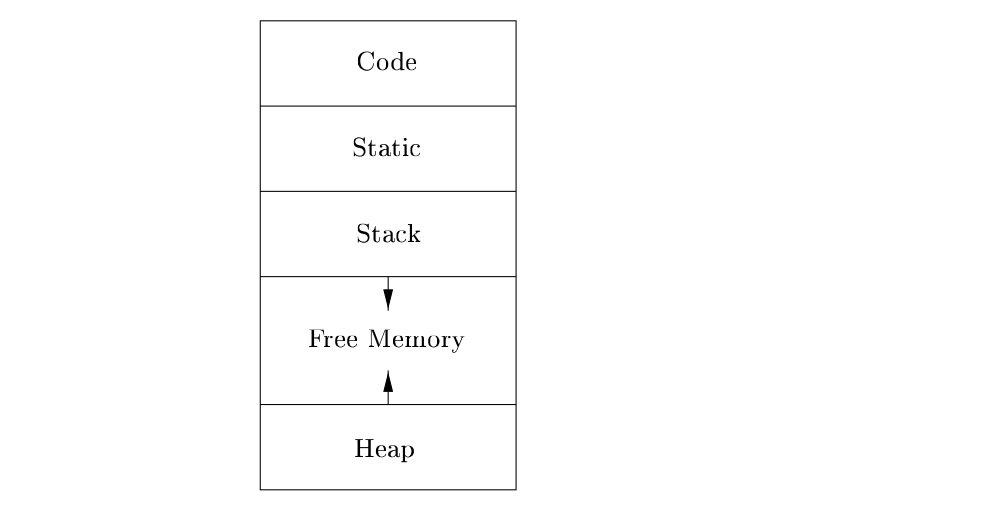
\includegraphics[width=0.5\textwidth,height=\textheight]{images/memory.png}
\caption{A program's memory segments roughly
classified}
\end{figure}

\begin{itemize}
\tightlist
\item
  In practice, the stack grows towards lower
  addresses, the heap towards higher(the diagram
  has it the other way around, but that doesn't
  matter).
\end{itemize}

\pause

\begin{itemize}
\tightlist
\item
  What are all these things ??
\end{itemize}

\pause

\begin{itemize}
\tightlist
\item
  We are mainly concerned withe the stack and the
  heap for the purpose of this talk, but we'll see
  what the other things are as well.
\end{itemize}
\end{frame}

\begin{frame}[fragile]{Code and Static segments}
\protect\hypertarget{code-and-static-segments}{}
\begin{itemize}
\tightlist
\item
  \textbf{Code}: Generated target code has a fixed
  size, allowing it to be stored in a statically
  determined area called Code, usually at the low
  end of memory.
\end{itemize}

\pause

\begin{itemize}
\tightlist
\item
  \textbf{Static}: Statically determined data
  objects, such as global constants and data
  generated by the compiler at compile time, can
  be stored in another area called Static.
\end{itemize}

\pause

\scriptsize

\begin{minted}[linenos,mathescape,breaklines,breakanywhere]{c}
const char* s = "Lorem Ipsum something something";
int main(){
  const char* string_arr[] = {"Made", "with", "love", "by", "Delta", "Force"};
  return 0;
}
\end{minted}

\normalsize

All the strings used in the above code segment are
stored in static section, while the instructions
generated for the program will be in code section.
\end{frame}

\begin{frame}[fragile]{Stack and Stack Allocation}
\protect\hypertarget{stack-and-stack-allocation}{}
\begin{itemize}
\tightlist
\item
  The stack will store things such as local
  variables, return address from a function call,
  etc.
\end{itemize}

\scriptsize

\begin{minted}[linenos,mathescape,breaklines,breakanywhere]{c}
int main(){
  int a = 10; // This is doing stack allocation
  int b = 20;
  int arr[2] = {1,2};
  return 0;
}
\end{minted}

\normalsize

\begin{figure}
\centering
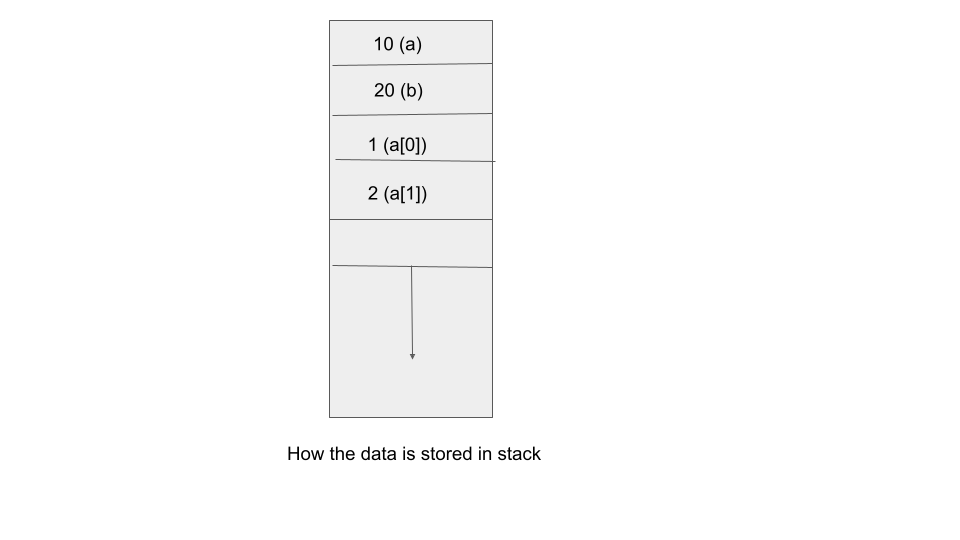
\includegraphics[width=0.5\textwidth,height=\textheight]{images/stack_layout.png}
\caption{Stack Layout for above code}
\end{figure}
\end{frame}

\begin{frame}[fragile]{Heap and Heap Allocation}
\protect\hypertarget{heap-and-heap-allocation}{}
\begin{itemize}
\tightlist
\item
  Many programming languages allow the programmer
  to allocate and deallocate data under program
  control.
\end{itemize}

\pause

\begin{itemize}
\tightlist
\item
  The heap is used to manage long-lived data.
\end{itemize}

\pause

\begin{itemize}
\tightlist
\item
  C/C++ has \texttt{malloc/realloc/free} functions
  for doing heap memory management.
\end{itemize}

\pause

\begin{itemize}
\tightlist
\item
  Unavoidable when we want to allocate memory
  whose size is known only when the program is
  running(dynamic allocation).
\end{itemize}

\pause

\scriptsize

\begin{minted}[linenos,mathescape,breaklines,breakanywhere]{c}
int* f(int n){
  return malloc(n*sizeof(int));
}
int main(){
   int n ;
   scanf("%d", &n);
   int *arr = f(n); // arr is heap allocated,returned from call to f
   free(arr); //Since, we're good programmers, we'll free the memory as well.
}
\end{minted}

\normalsize
\end{frame}

\begin{frame}[fragile]{What exactly are
malloc/realloc/free?}
\protect\hypertarget{what-exactly-are-mallocreallocfree}{}
Heap allocation functions:

\begin{itemize}
\tightlist
\item
  \texttt{\textcolor{red}{malloc(x)} }: allocate
  \passthrough{\lstinline!x!} bytes in heap
\end{itemize}

\pause

\begin{itemize}
\tightlist
\item
  \texttt{\textcolor{red}{ realloc(p, x) }}:
  resize previously allocated heap memory
\end{itemize}

\pause

\begin{itemize}
\tightlist
\item
  \texttt{\textcolor{red}{ free(p) } }: return
  heap memory to the operating system
\end{itemize}
\end{frame}

\hypertarget{introduction-to-memory-management}{%
\section{Introduction to Memory
Management}\label{introduction-to-memory-management}}

\begin{frame}{Introduction to Memory Management}
\begin{itemize}
\tightlist
\item
  Memory management is all about using
  \texttt{heap memory} correctly.
\end{itemize}

\pause

\begin{itemize}
\tightlist
\item
  If it's done incorrectly, the program can
  \textcolor{red}{crash } or
  \textcolor{red}{slow down}.
\end{itemize}

\pause

\begin{itemize}
\tightlist
\item
  Stack allocations don't need to be freed;
  they're automatically managed with
  \textbf{scopes} (we'll talk about scopes in the
  next slide).
\end{itemize}

\pause

\begin{itemize}
\tightlist
\item
  There are different techniques for managing heap
  memory.
\end{itemize}

\begin{block}{Important terminology}
\protect\hypertarget{important-terminology}{}
\begin{itemize}
\tightlist
\item
  \textbf{\textcolor{red}{Memory Leak}}: It
  happens when you ask the operating system for
  memory but don't return it back.
\end{itemize}
\end{block}
\end{frame}

\begin{frame}[fragile]{What is this scope thing??}
\protect\hypertarget{what-is-this-scope-thing}{}
\scriptsize

\begin{minted}[linenos,mathescape,breaklines,breakanywhere]{cpp}
// NOTE: This function won't compile
int f(){ // scope '1 starts
    int a = 10;
    { // scope '2 starts
       int b = 20;
    } // scope '2 ends
    if(a == 10){ // scope '3 starts
      int c = 30;
    } // scope '3 ends
    return b; // This fails because it's not in scope
} // scope '1 ends
\end{minted}

\normalsize
\end{frame}

\begin{frame}{Why should I care about freeing
memory? Is it really a problem?}
\protect\hypertarget{why-should-i-care-about-freeing-memory-is-it-really-a-problem}{}
\begin{itemize}
\tightlist
\item
  If your system has infinite memory, you don't
  need to worry. However, since memory is finite,
  you must take care. \pause
\item
  If one program uses up all the memory, other
  programs that require memory won't be able to
  function properly. \pause
\item
  Your program may \textcolor{red}{crash} if it
  requests more memory than the operating system
  can provide. \pause
\item
  Memory leaks can have a significant impact on
  long-running programs such as
  \texttt{web servers, editors, and IDEs}.
\end{itemize}
\end{frame}

\hypertarget{ways-to-manage-memory}{%
\section{Ways to manage
memory}\label{ways-to-manage-memory}}

\begin{frame}{Ways to manage memory}
We have two ways to do memory management.

\pause

\begin{itemize}
\item
  \textbf{Manual Memory Management} : Languages
  such as C, C++, Rust, etc have this
\item
  \textbf{Automatic Memory Management}: Languages
  such as Python, Java, Go, JavaScript, Swift, etc
  have this.
\end{itemize}
\end{frame}

\hypertarget{manual-memory-management}{%
\section{Manual Memory
Management}\label{manual-memory-management}}

\begin{frame}[fragile]{Scenarios where you can go
wrong}
\protect\hypertarget{scenarios-where-you-can-go-wrong}{}
\begin{columns}[T]
\begin{column}{0.4\textwidth}
\vspace{30pt}
\tiny

\begin{minted}[linenos,mathescape,breaklines,breakanywhere]{cpp}
// NOTE: this is a dumb example to show where things can go wrong,
// I don't actually write code like this
int* allocate_and_throw_exn_if_n_lt_10(int n){
   int *arr = malloc(n*sizeof(int));
   if (n < 10){
       throw runtime_error("n < 10");
   }
   return arr;
}
int main(){
    try {
        auto *arr = allocate_and_throw_exn_if_n_lt_10(2);
        free(arr);
    } catch(const std::runtime_error &e){
        cout << "Error:" <<e.what() << endl;
    }
}
\end{minted}

\normalsize
\end{column}

\begin{column}{0.6\textwidth}
\begin{figure}
\centering
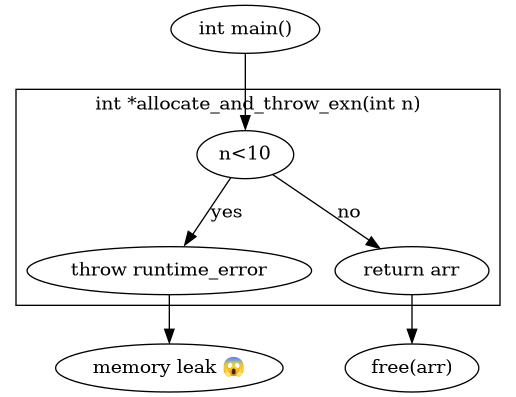
\includegraphics[width=0.7\textwidth,height=\textheight]{images/mem_management_leak_scenario1.png}
\caption{Flow for the leaking code}
\end{figure}

\begin{figure}
\centering
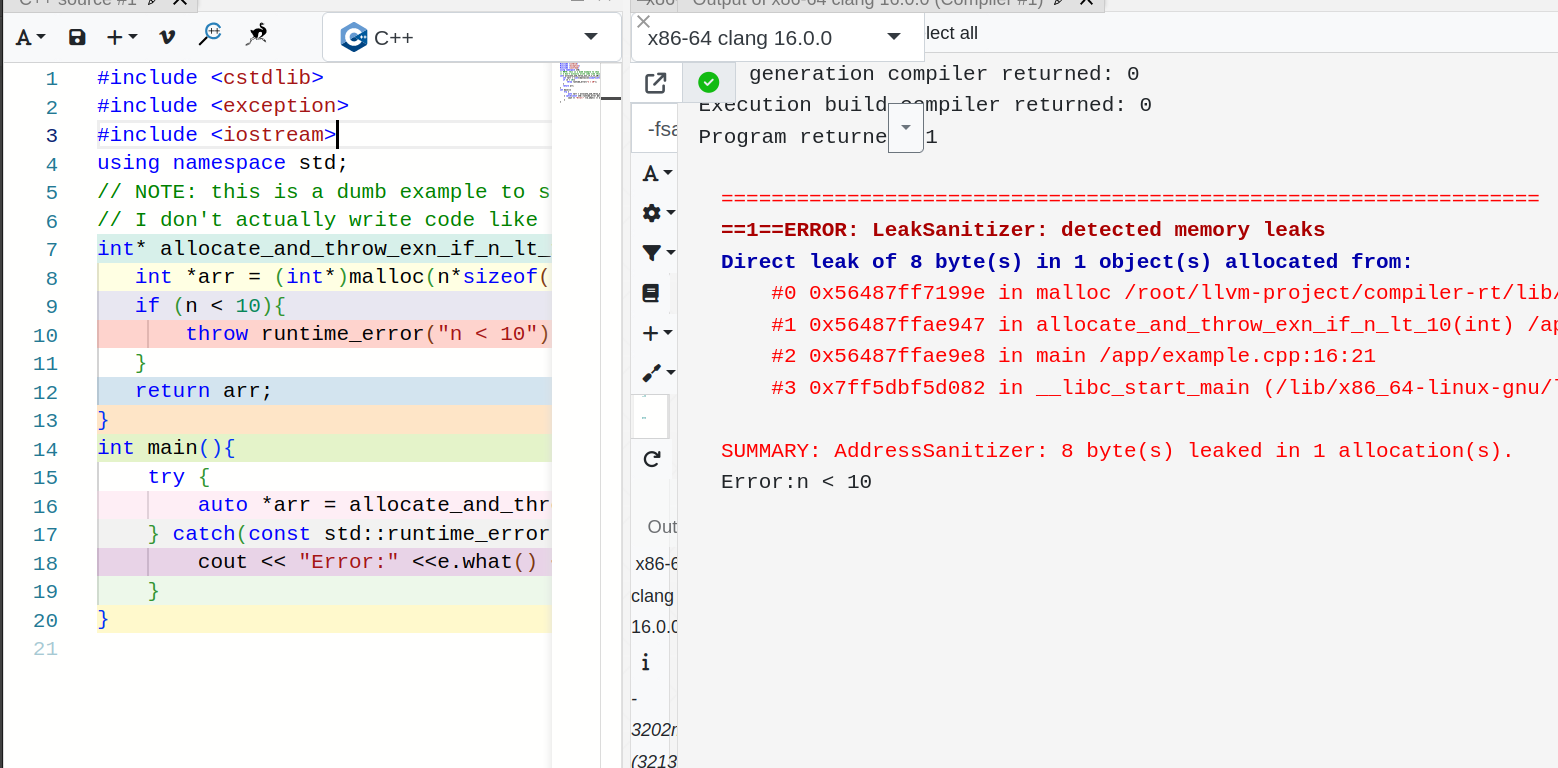
\includegraphics[width=0.9\textwidth,height=\textheight]{images/./leak_detected.png}
\caption{Memory Leak Detected by address
sanitizer}
\end{figure}
\end{column}
\end{columns}
\end{frame}

\begin{frame}{How to fix it??}
\protect\hypertarget{how-to-fix-it}{}
\begin{itemize}
\item
  \textcolor{red}{DON'T WRITE DUMB CODE LIKE I DID}
\item
  More high level language(than C) like C++, Rust
  provide us with smart ways to manage memory
\item
  They come built-in with smart pointer types like
  \texttt{unique\textunderscore ptr} (C++)
\end{itemize}
\end{frame}

\begin{frame}[fragile]{Fixing the code with smart
pointer}
\protect\hypertarget{fixing-the-code-with-smart-pointer}{}
\scriptsize

\begin{columns}[T]
\begin{column}{0.48\textwidth}
\begin{minted}[linenos,mathescape,breaklines,breakanywhere]{cpp}
std::unique_ptr<int[]> allocate_and_throw_exn_if_n_lt_10(int n){
   auto *arr = make_unique<int[]>(new int[n]);
   if (n < 10){
       throw runtime_error("n < 10");
   }
   return arr;
}
int main(){
    try {
        auto arr = allocate_and_throw_exn_if_n_lt_10(2);
    } catch(const std::runtime_error &e){
        cout << "Error:" <<e.what() << endl;
    }
}
\end{minted}

\normalsize

\pause
\end{column}

\begin{column}{0.48\textwidth}
\vspace{90pt}

\begin{center}

\large
\textbf{\textcolor{red}{What the hell just happened??}}

\normalsize

We're not even freeing anything?? How does this work?

\end{center}
\end{column}
\end{columns}
\end{frame}

\begin{frame}{How do smart pointers work?}
\protect\hypertarget{how-do-smart-pointers-work}{}
\begin{columns}[T]
\begin{column}{0.3\textwidth}
\vspace{20pt}

\begin{itemize}
\tightlist
\item
  Uses \textbf{scope} to track lifetime of a
  pointer(scopes mentioned in
  \protect\hyperlink{what-is-this-scope-thing}{previous
  section})
\end{itemize}

\pause

\begin{itemize}
\tightlist
\item
  C++ uses \texttt{destructors} to run code when
  an object goes out of scope. (due to RAII in
  C++)
\end{itemize}

\pause
\end{column}

\begin{column}{0.7\textwidth}
\begin{block}{What is RAII in C++?}
\protect\hypertarget{what-is-raii-in-c}{}
\begin{figure}
\centering
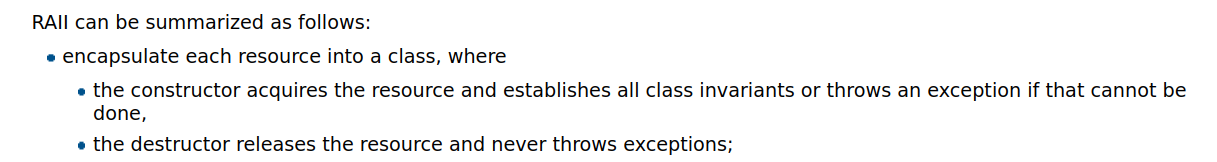
\includegraphics{images/raii.png}
\caption{RAII}
\end{figure}

\begin{figure}
\centering
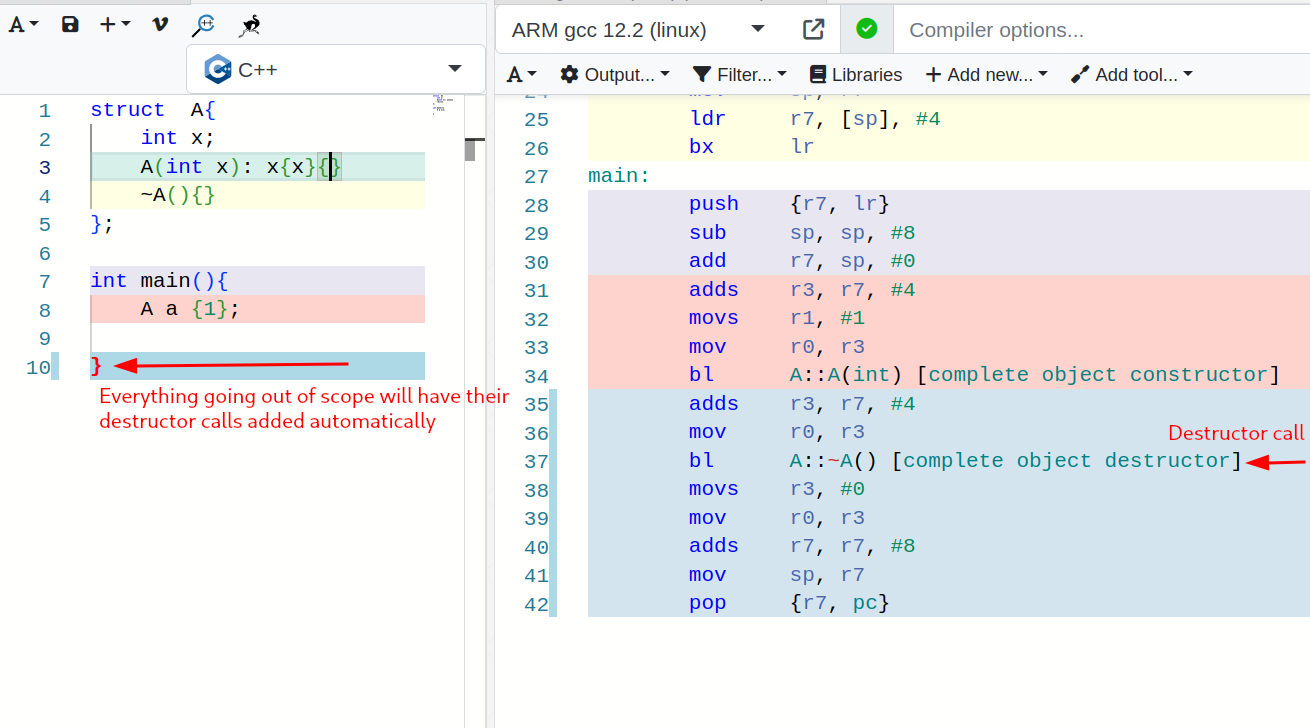
\includegraphics{images/./destructor.png}
\caption{Destructor call added automatically}
\end{figure}
\end{block}
\end{column}
\end{columns}
\end{frame}

\begin{frame}[fragile]{Let's make our own
unique\_ptr}
\protect\hypertarget{lets-make-our-own-unique_ptr}{}
\begin{columns}[T]
\begin{column}{0.48\textwidth}
\scriptsize

\begin{minted}[linenos,mathescape,breaklines,breakanywhere]{cpp}
#include <iostream>
using namespace std;
class int_ptr{
    int* x ;
public:
    int_ptr(int x): x{new int(x)}{}
    ~int_ptr(){
        delete x;
    }
    int& operator*(){
        return *x;
    }
};
int main(){
    int_ptr one(1);
    cout << *one << endl;
}
\end{minted}

\normalsize
\end{column}

\begin{column}{0.48\textwidth}
\vspace{30pt}

\begin{figure}
\centering
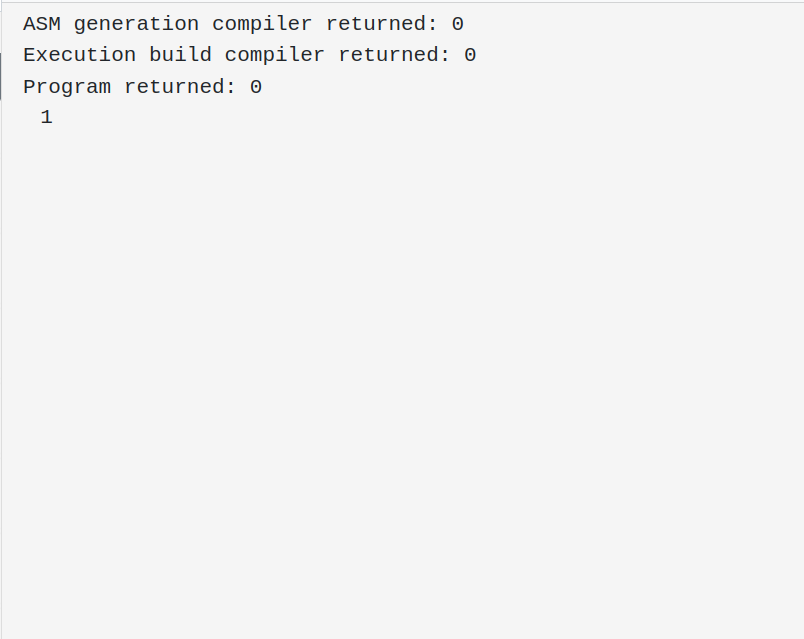
\includegraphics{images/./int_ptr_working.png}
\caption{int\_ptr working without any leaks}
\end{figure}
\end{column}
\end{columns}
\end{frame}

\begin{frame}{Is unique\_ptr the only smart
pointer??}
\protect\hypertarget{is-unique_ptr-the-only-smart-pointer}{}
\huge

\centering\textbf{\textcolor{red}{ NO }}
\normalsize
\end{frame}

\begin{frame}{Isn't unique\_ptr perfect already?
Why would I need anything else?}
\protect\hypertarget{isnt-unique_ptr-perfect-already-why-would-i-need-anything-else}{}
\begin{itemize}
\tightlist
\item
  Problem with \texttt{unique\textunderscore ptr}
  is that it can have only one owner.
\end{itemize}

\pause

\begin{columns}[T]
\begin{column}{0.3\textwidth}
\begin{block}{Case in Point}
\protect\hypertarget{case-in-point}{}
\begin{itemize}
\tightlist
\item
  A \texttt{unix file descriptor}
\end{itemize}

\pause

\begin{itemize}
\tightlist
\item
  A file descriptor can have multiple owners. It
  should only be freed when all the owners go out
  of scope.
\end{itemize}
\end{block}
\end{column}

\begin{column}{0.7\textwidth}
\pause

\begin{figure}
\centering
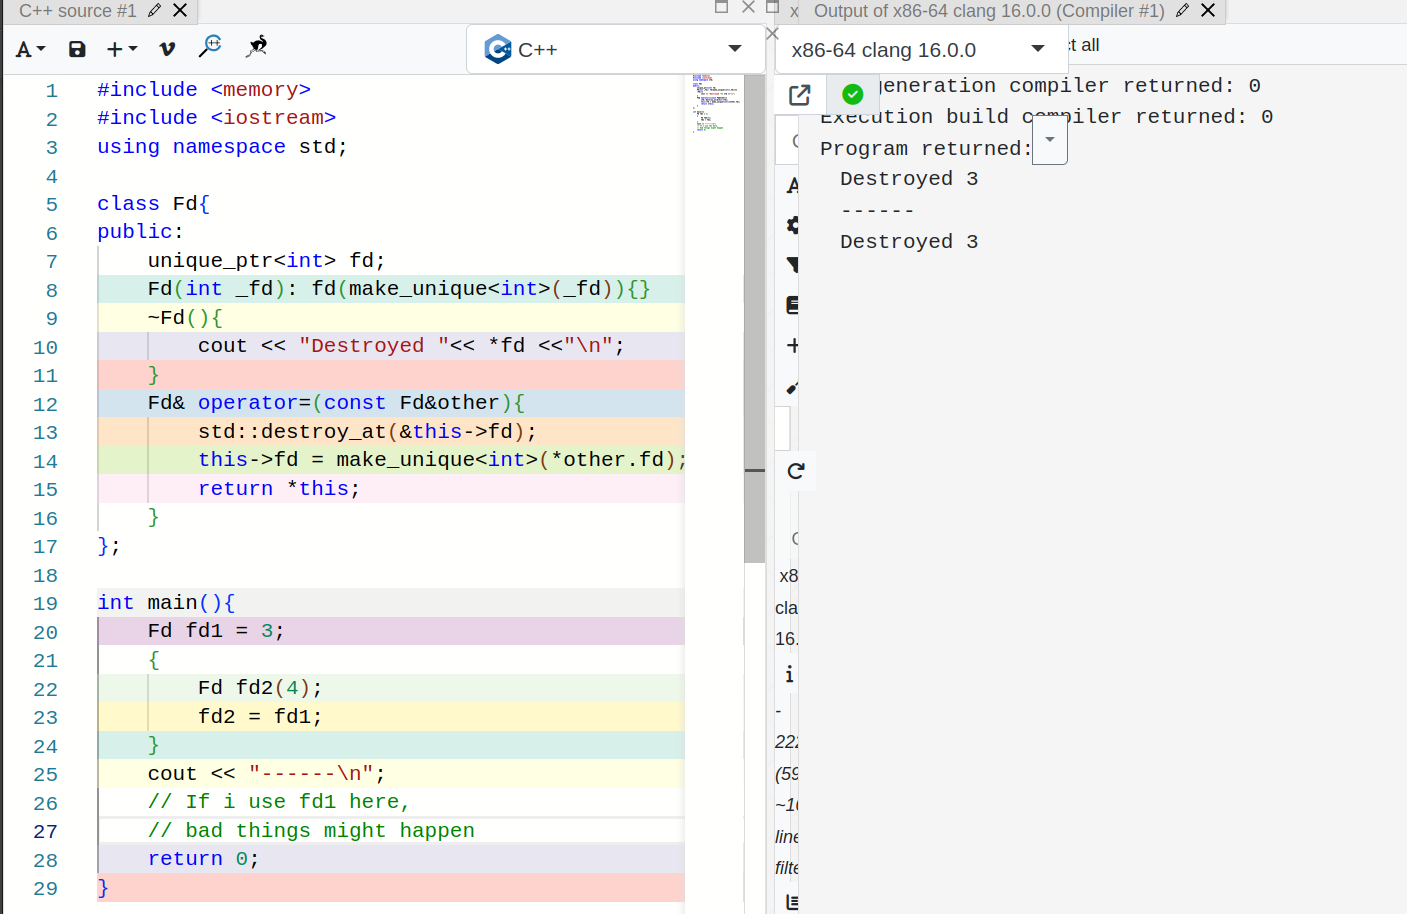
\includegraphics{images/./fd.png}
\caption{File Descriptor with unique\_ptr(the code
is very bad🥲)}
\end{figure}
\end{column}
\end{columns}

\pause

\centering {\textbf{Not possible to model this correctly }}

\pause

\centering {\textbf{That's why we need more }}
\end{frame}

\hypertarget{introduction-to-automatic-memory-management}{%
\section{Introduction to Automatic Memory
Management}\label{introduction-to-automatic-memory-management}}

\hypertarget{reference-counting}{%
\section{Reference
Counting}\label{reference-counting}}

\hypertarget{trace-based-collection}{%
\section{Trace Based
Collection}\label{trace-based-collection}}

\hypertarget{which-is-betterautomatic-memory-management-or-manual-management}{%
\section{Which is better?(Automatic Memory
Management or Manual
Management}\label{which-is-betterautomatic-memory-management-or-manual-management}}

\hypertarget{advanced-topics-in-garbage-collection}{%
\section{Advanced Topics in Garbage
Collection}\label{advanced-topics-in-garbage-collection}}

\begin{frame}{Advanced Topics in Garbage
Collection}
\begin{itemize}
\item
  Incremental GC
\item
  Parallel and Concurrent GC
\item
  Precise and Conservative Garbage Collectors
\item
  Reducing GC pause*
\end{itemize}
\end{frame}

\hypertarget{references}{%
\section{References}\label{references}}

\begin{frame}{References}
\begin{itemize}
\tightlist
\item
  \href{https://rebelsky.cs.grinnell.edu/Courses/CS302/99S/Presentations/GC/}{Some
  presentation on GC, Grinnel college}
\end{itemize}
\end{frame}

\end{document}
